\documentclass[12pt]{article}
\usepackage{graphicx}
\usepackage{ltcadiz}
\usepackage{listings}
\usepackage{amssymb}
\lstset{breaklines=true, numbers=left}

\title{Report on OGO 2.2 Softwarespecification\\ Assignment 2a}
\author{
        Tim van Dalen, Tony Nan, Ferry Timmers, \\ Lasse Blaauwbroek, Femke Jansen, \\Jeroen Peters and Sander Breukink\\ OGO 2.2 group 6 \\
                Department of Computer Science\\
        Technical University Eindhoven\\
}
\date{\today}

\begin{document}

\maketitle

\begin{abstract}
\end{abstract}

\section{Introduction}

In this document we give an (informal) specification of a board game.
The game will take base around a set of islands (or a single one)
in the middle of an ocean far away. On the island a group of foxes
lives that by evolution have acquired a taste for dolphins that live
in the nearing ocean. The dolphins in turn have acquired a taste of
the foxes because this area of the sea has not enough fish for them
to feed on. The tides in this area of the world are very unpredictable
and therefore it can catch the foxes and dolphins by surprise. The
dolphins can only move in the water and beaches; the foxes can only
move on land and shores. When a fox is in the water or a dolphin is
on the land it will be an easy victim since it can not move.

In the game there are two players, one commands the foxes and the
other the dolphins. Both animals have a territory that can not be
visited by animals of the same player because they will get in a fight.
When a fox visits a territory of a dolphin he will eat him, this also
works the other way around. The objective of each player is to eat
all animals of the opponent before his own are eaten.

To make the game more exiting there are also bridges and water caves;
the bridges can only be crossed by foxes and the water caves by dolphins.
There are also two events that make the tides more advantageous for
the players. The wet season will create higher tides and the dry season
will create lower tides.

\section{Structure}

The assignment is to develop a game. The game is being played by two computer 
aided players on a board that consists of tiles. \\
Thus, the game consists of four parts, the two players, a board and the view.\\
To make sure that these parts can communicate with each other a controller has 
to be made. This controller receives requests of the players on which it replies. 
It then updates the state of the game by making requests to the board. 
The board can choose to deny a request if it isn't legal by the rules of the game.\\
The game should be shown real-time on a screen, which is handled by the view component. 
The view component draw the state of the board on the screen.\\
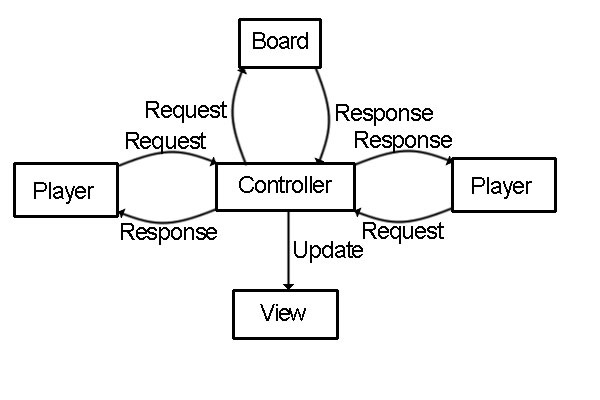
\includegraphics{plaatje-2a}
It is not mandatory to separate this functionality from the controller, 
but it would be appreciated.\\
The board can also update its own state between two rounds, to make events possible. 
Because of this it is not possible to use locally stored user-data, as this data 
doesn't have to be up to date: only the game-situation on the board has to be correct.\\


\section{Game}

\subsection{Playing field}

The playing field consists of a two-dimensional grid of hexagonal tiles. Every tile has an associated elevation value which can be represented using color. Some of the tiles are flooded with water (depending on their elevation) and the other tiles are land. Initially, the tiles with land have to be adjacent. Two adjacent tiles (meaning they have a common edge) may only differ in two units of elevation. We can have bridges and underwater caves between two tiles. A dolphin can swim across a cave as long as both endpoints are flooded and a fox can cross a bridge as long as both endpoints are not flooded.

The elevation of a tile lies between minus fifty and fifty. The sum of the elevation of all tiles must be zero. The water elevation lies between minus fifteen and fifteen and is initially zero. The tide of the water determines the exact elevation. The tide can randomly change between rounds and changes between one and five elevation units. The speed of propagation of water is two tiles per round (in the natural direction of the propagation).

A safe tile for a fox has an elevation of more than fifteen and a safe tile for a dolphin has an elevation of less than minus fifteen.

\subsection{Gameplay}
There are two players, each of them controlling a set of dolphins or a set of foxes. Initially there are an equal number of foxes and dolphins. This number can be defined beforehand by the players. The size of the playing board is dependent on the initial number of animals.

All dolphins are initially placed in the water and all foxes are initially placed on land. No two animals of the same type can reside on the same tile.

The game is played in rounds. In every round each player can move one quarter of the total number of animals at that moment in the game. A move means that one animal can move from one tile to an adjacent tile (or cross a bridge or cave). The player can determine how he distributes his moves between his animals. After a round the computer can adjust the tide level and let the water propagate accordingly.

A fox in the water can be eaten by a dolphin on the same tile. The fox vanishes from the board when this happens. When a fox is further than two tiles away from the land it cannot move until the tide drops again. Similarly, a dolphin on the land can be eaten by a fox and if it is more than two tiles away from the water it cannot move until the tide rises again.

The game has ended when one of the players has no animals left.

\subsection{Natural events}
Between two rounds a natural event can occur. Those events are the dry season and the wet season. These seasons can shift the maximum and minimum value of the tide with a maximum of twenty units. Dry season means the shift is negative and wet season means the shift is positive. A season lasts for five rounds. A natural event occurs with a probability of five percent. And no two natural events can occur a the same time.

\end{document}
